\documentclass[12pt,a4paper]{report}
\usepackage[utf8]{inputenc}
\usepackage{graphicx}
\usepackage{amsmath,amssymb}
\usepackage{setspace}
\usepackage{hyperref}
\hypersetup{
    colorlinks=true,
    linkcolor=blue,
    filecolor=magenta,
    urlcolor=cyan,
    citecolor=red,
    pdftitle={Early Disease Detection in Chicken Using Audio-Based Deep Learning},
    pdfpagemode=FullScreen,
}
\usepackage{geometry}
\usepackage{xcolor}
\usepackage{listings}
\usepackage{booktabs}
\usepackage{multirow}
\usepackage{array}
\usepackage{float}
\usepackage{subcaption}
% Listings package configuration
\lstset{
  basicstyle=\small\ttfamily,
  columns=flexible,
  breaklines=true,
  keywordstyle=\bfseries\color{blue},
  commentstyle=\itshape\color{teal},
  stringstyle=\color{purple},
  showstringspaces=false,
  numbers=left,
  numberstyle=\tiny\color{gray},
  frame=single,
  rulecolor=\color{black},
  backgroundcolor=\color{gray!10}
}

% Page geometry setup
\geometry{
  left=1in,
  right=1in,
  top=1in,
  bottom=1in
}

% Set line spacing to one and a half
\onehalfspacing

% Figure paths
\graphicspath{{cnn_model/results/}}

\begin{document}

%%%%%%%%%%%%%%%%%%%%%%%%%%%%%%%%%%%%%%%%%%%%%%%%%%%%%%%%%%%%%%
% Title Page
%%%%%%%%%%%%%%%%%%%%%%%%%%%%%%%%%%%%%%%%%%%%%%%%%%%%%%%%%%%%%%
\begin{titlepage}
    \centering
    \vspace*{3cm}

    % Title
    {\Large\textbf{Early Disease Detection in Chicken\\Using Audio-Based Deep Learning}\\[1.5em]
    \normalsize B.Tech Project Report}\\[3em]

    % Submitted by section
    \textbf{Submitted by}\\
    \large \textbf{Sohel Akhtar}\\
    \normalsize (Roll No.: 2301216)\\[2em]

    % Guidance section
    \textbf{Under the Guidance of}\\
    \large Prof. Ferdous Ahmed Barbhuiya\\[3em]

    % Institute Logo
    \includegraphics[width=10cm]{iiitg.png} \\[1em]

    % Department and Institute Name
    Department of Computer Science and Engineering\\
    Indian Institute of Information Technology Guwahati \\[1em]

    \vfill
\end{titlepage}

%%%%%%%%%%%%%%%%%%%%%%%%%%%%%%%%%%%%%%%%%%%%%%%%%%%%%%%%%%%%%%
% Declaration
%%%%%%%%%%%%%%%%%%%%%%%%%%%%%%%%%%%%%%%%%%%%%%%%%%%%%%%%%%%%%%
\chapter*{Declaration}
\label{sec:declaration}
\addcontentsline{toc}{chapter}{Declaration}

\vspace*{1em}

I, \textbf{Sohel Akhtar}, hereby declare that the work presented in this B.Tech project report, titled \emph{``Early Disease Detection in Chicken Using Audio-Based Deep Learning''}, is my original work and has not been submitted in the same form to any other institution or university for the award of any degree or diploma. Wherever contributions of others are involved, they have been appropriately cited and acknowledged.

\vspace*{4em}

\noindent
Signature: \rule{6cm}{0.4pt}\\[2em]
Name: Sohel Akhtar\\[1em]
Roll No.: 2301216\\[2em]

\noindent
Date: \rule{6cm}{0.4pt}

\clearpage

%%%%%%%%%%%%%%%%%%%%%%%%%%%%%%%%%%%%%%%%%%%%%%%%%%%%%%%%%%%%%%
% Certificate
%%%%%%%%%%%%%%%%%%%%%%%%%%%%%%%%%%%%%%%%%%%%%%%%%%%%%%%%%%%%%%
\chapter*{Certificate}
\label{sec:certificate}
\addcontentsline{toc}{chapter}{Certificate}

\vspace*{1em}

This is to certify that the B.Tech project report entitled \emph{``Early Disease Detection in Chicken Using Audio-Based Deep Learning''}, submitted by \textbf{Sohel Akhtar} (Roll No. 2301216), has been carried out under my supervision. To the best of my knowledge, this work embodies the student's own research efforts and has not been submitted elsewhere for any degree or diploma.

\vspace*{4em}

\noindent
\rule{6cm}{0.4pt}\\
\noindent Prof. Ferdous Ahmed Barbhuiya\\
Department of Computer Science and Engineering\\
Indian Institute of Information Technology Guwahati

\clearpage

%%%%%%%%%%%%%%%%%%%%%%%%%%%%%%%%%%%%%%%%%%%%%%%%%%%%%%%%%%%%%%
% Acknowledgements
%%%%%%%%%%%%%%%%%%%%%%%%%%%%%%%%%%%%%%%%%%%%%%%%%%%%%%%%%%%%%%
\chapter*{Acknowledgements}
\label{sec:acknowledgements}
\addcontentsline{toc}{chapter}{Acknowledgements}

\vspace*{1em}

I wish to express my sincere gratitude to my project supervisor, \textbf{Prof. Ferdous Ahmed Barbhuiya}, for his invaluable guidance, consistent support and insightful feedback throughout the duration of this project. His encouragement was instrumental in navigating the challenges encountered.

I am also thankful to the \textbf{Department of Computer Science and Engineering} at the Indian Institute of Information Technology Guwahati for providing the necessary computational resources, infrastructure, and academic environment essential for this research.

Finally, I extend my appreciation to my family, friends and peers for their unwavering support, understanding and motivation, which were crucial during this demanding period.

\clearpage

%%%%%%%%%%%%%%%%%%%%%%%%%%%%%%%%%%%%%%%%%%%%%%%%%%%%%%%%%%%%%%
% Abstract
%%%%%%%%%%%%%%%%%%%%%%%%%%%%%%%%%%%%%%%%%%%%%%%%%%%%%%%%%%%%%%
\chapter*{Abstract}
\label{sec:abstract}
\addcontentsline{toc}{chapter}{Abstract}

\vspace*{1em}

Respiratory diseases are a leading cause of mortality in poultry farms, responsible for 30--40\% of flock losses. Early detection of these diseases is critical for effective treatment and minimizing economic damage. This report presents an automated, non-invasive system for early disease detection in chickens based on audio analysis of their vocalizations using deep learning.

The proposed system employs a comprehensive audio processing pipeline that includes Hamming windowing for spectral leakage reduction, low-pass filtering for noise suppression, and extraction of a rich 243-dimensional feature vector encompassing Mel-Frequency Cepstral Coefficients (MFCCs), Delta MFCCs, Chroma features, Mel spectrogram statistics, Spectral Contrast, Tonnetz, and various spectral and statistical descriptors. These features are fed into a 1D Convolutional Neural Network (CNN) architecture incorporating ResNet-style skip connections and an attention mechanism, designed to classify audio signals into three categories: Healthy, Noise, and Unhealthy.

To address model variance and improve generalization, a 3-model ensemble strategy is adopted, where predictions from three independently trained CNN models are averaged. The system was trained and evaluated on a dataset of 344 poultry vocalization recordings sampled at 96~kHz. The single best CNN model achieved a test accuracy of 74.5\%, while the ensemble approach significantly boosted performance to \textbf{92.8\%} overall accuracy, with per-class recall of 91.6\% for Healthy, 90.4\% for Noise, and 95.9\% for Unhealthy vocalizations. The high recall for the Unhealthy class is particularly significant for practical deployment in disease monitoring systems.

\clearpage

%%%%%%%%%%%%%%%%%%%%%%%%%%%%%%%%%%%%%%%%%%%%%%%%%%%%%%%%%%%%%%
% Table of Contents
%%%%%%%%%%%%%%%%%%%%%%%%%%%%%%%%%%%%%%%%%%%%%%%%%%%%%%%%%%%%%%
\tableofcontents
\clearpage
\listoffigures
\addcontentsline{toc}{chapter}{List of Figures}
\clearpage
\listoftables
\addcontentsline{toc}{chapter}{List of Tables}
\clearpage

%%%%%%%%%%%%%%%%%%%%%%%%%%%%%%%%%%%%%%%%%%%%%%%%%%%%%%%%%%%%%%
% Chapter 1: Introduction
%%%%%%%%%%%%%%%%%%%%%%%%%%%%%%%%%%%%%%%%%%%%%%%%%%%%%%%%%%%%%%
\chapter{Introduction}
\label{ch:intro}

\section{Background}

The global poultry industry is one of the largest and fastest-growing segments of the agricultural sector, providing a major source of protein for billions of people worldwide. However, poultry farming faces significant challenges from respiratory diseases, which are among the most devastating health issues affecting commercial flocks. Diseases such as infectious bronchitis, Newcastle disease, avian influenza, and chronic respiratory disease (caused by \textit{Mycoplasma gallisepticum}) can spread rapidly through a flock, causing mortality rates of 30--40\% if not detected and treated early \cite{datainbrief2023}.

Traditional disease detection methods rely heavily on manual inspection by trained veterinarians or farm workers, who listen for abnormal sounds such as coughing, snoring, rales (crackling sounds), and gasping. While effective, this approach is inherently limited by several factors:
\begin{itemize}
    \item \textbf{Scalability:} Modern poultry farms may house tens of thousands of birds, making individual monitoring impractical.
    \item \textbf{Subjectivity:} Human perception varies, and subtle early-stage disease sounds may be missed.
    \item \textbf{Timeliness:} Periodic inspection cannot provide the continuous, real-time monitoring needed for early intervention.
    \item \textbf{Cost:} Employing sufficient trained personnel for round-the-clock monitoring is economically prohibitive.
\end{itemize}

\section{Motivation}

Audio-based monitoring offers a compelling alternative: it is \textbf{non-invasive} (no physical contact with birds is required), can operate \textbf{continuously in real-time}, and can be deployed using relatively inexpensive microphone hardware. The key insight is that respiratory diseases produce characteristic changes in chicken vocalizations --- healthy chickens produce regular clucking and cooing sounds, while diseased birds exhibit coughing, snoring, and rales that have distinct spectral signatures.

Recent advances in deep learning, particularly Convolutional Neural Networks (CNNs), have demonstrated remarkable success in audio classification tasks across domains such as speech recognition, music genre classification, and environmental sound detection. These methods can automatically learn discriminative patterns from audio features without requiring hand-crafted rules, making them well-suited for the poultry health classification problem.

\section{Objectives}

The primary objectives of this project are:
\begin{enumerate}
    \item To develop a robust audio preprocessing pipeline that reduces noise while preserving disease-indicative vocal features.
    \item To design a comprehensive feature extraction framework that captures the acoustic characteristics distinguishing healthy, unhealthy, and noise signals.
    \item To build and train a 1D CNN model with ResNet-style skip connections and attention mechanisms for poultry health classification.
    \item To implement an ensemble strategy that improves classification accuracy and reduces model variance.
    \item To evaluate the system's performance and demonstrate its potential for real-world deployment in poultry farms.
\end{enumerate}

\section{Report Organization}

The remainder of this report is organized as follows:
\begin{itemize}
    \item \textbf{Chapter 2: Literature Review} --- Reviews existing work on poultry vocalization analysis, audio classification, and related machine learning approaches.
    \item \textbf{Chapter 3: Problem Statement} --- Formally defines the classification problem and describes the dataset.
    \item \textbf{Chapter 4: Proposed System} --- Details the complete system architecture including preprocessing, feature extraction, and the CNN model.
    \item \textbf{Chapter 5: Results} --- Presents experimental results with analysis.
    \item \textbf{Chapter 6: Conclusion and Future Work} --- Summarizes findings and outlines future directions.
\end{itemize}


%%%%%%%%%%%%%%%%%%%%%%%%%%%%%%%%%%%%%%%%%%%%%%%%%%%%%%%%%%%%%%
% Chapter 2: Literature Review
%%%%%%%%%%%%%%%%%%%%%%%%%%%%%%%%%%%%%%%%%%%%%%%%%%%%%%%%%%%%%%
\chapter{Literature Review}
\label{ch:literature_review}

\section{Audio-Based Poultry Health Monitoring}

The use of audio signals for monitoring poultry health has gained significant research attention in recent years. The \textit{Data in Brief} (Volume 50, 2023) \cite{datainbrief2023} published a comprehensive Poultry Vocalization Signal Dataset that includes recordings of healthy and diseased chickens. The dataset employs Hamming windowing and Kalman filtering as preprocessing steps to reduce spectral leakage and denoise signals while preserving disease-indicative markers. This dataset forms the foundation of our work.

Audio-based systems offer distinct advantages over visual or sensor-based methods: they do not require physical contact with the birds, can cover large areas with relatively few microphones, and can operate continuously without disturbing the flock.

\section{Feature Extraction from Audio Signals}

\textbf{Mel-Frequency Cepstral Coefficients (MFCCs)} have been the dominant feature representation in audio classification tasks since their introduction for speech recognition. MFCCs approximate the human auditory system's frequency response using a mel-scale filterbank, making them effective at capturing vocal tract characteristics. Prior work in poultry health classification has primarily relied on MFCC features, sometimes supplemented with basic spectral descriptors \cite{datainbrief2023}.

However, relying solely on MFCCs may miss important disease markers. Recent studies have demonstrated that combining MFCCs with additional features such as:
\begin{itemize}
    \item \textbf{Delta MFCCs:} Temporal derivatives that capture dynamic changes in the spectral envelope.
    \item \textbf{Chroma features:} Represent pitch class profiles useful for tonal analysis.
    \item \textbf{Spectral contrast:} Measures the difference between spectral peaks and valleys across frequency bands.
    \item \textbf{Tonnetz:} Captures tonal centroid features representing harmonic relationships.
\end{itemize}
can significantly improve classification performance by providing a more complete acoustic characterization.

\section{Machine Learning Approaches}

Traditional machine learning approaches for audio classification include Support Vector Machines (SVMs), Random Forests, and Gradient Boosting methods. XGBoost \cite{chen2016xgboost}, in particular, has shown strong performance on tabular feature data due to its regularized gradient boosting framework. However, these methods require careful feature engineering and may not fully exploit the complex patterns present in high-dimensional audio feature spaces.

Deep learning approaches, particularly CNNs, have shown superior performance in audio classification by automatically learning hierarchical feature representations. Key architectural innovations that have proven beneficial include:
\begin{itemize}
    \item \textbf{Residual connections (ResNet):} Enable training of deeper networks by allowing gradient flow through skip connections \cite{he2016resnet}.
    \item \textbf{Attention mechanisms:} Allow the model to focus on the most informative parts of the input, improving discrimination between similar classes.
    \item \textbf{Ensemble methods:} Combining predictions from multiple models reduces variance and improves robustness.
\end{itemize}

\section{Gaps in Existing Work}

Despite the progress made, several gaps remain in the existing literature:
\begin{itemize}
    \item \textbf{Limited feature sets:} Most existing systems use only MFCC features, ignoring potentially discriminative features from the power spectrum, spectral contrast, and tonnetz domains.
    \item \textbf{Class imbalance:} Many studies do not adequately address the imbalanced distribution of healthy vs. unhealthy samples typical of real-world datasets.
    \item \textbf{Model robustness:} Single-model approaches are susceptible to overfitting, especially on small datasets, and lack the robustness needed for deployment.
    \item \textbf{Preprocessing limitations:} While Kalman filtering is theoretically optimal for denoising, its computational cost makes it impractical for real-time, large-scale processing.
\end{itemize}

This project addresses these gaps by developing a comprehensive 243-dimensional feature set, employing a computationally efficient preprocessing pipeline, and using a CNN ensemble for robust classification.


%%%%%%%%%%%%%%%%%%%%%%%%%%%%%%%%%%%%%%%%%%%%%%%%%%%%%%%%%%%%%%
% Chapter 3: Problem Statement
%%%%%%%%%%%%%%%%%%%%%%%%%%%%%%%%%%%%%%%%%%%%%%%%%%%%%%%%%%%%%%
\chapter{Problem Statement}
\label{ch:problem_statement}

\section{Task Definition}

The task addressed in this project is the \textbf{automatic classification of poultry audio signals} into one of three predefined categories based on the acoustic content of the recording:

\begin{itemize}
    \item \textbf{Input:} A raw audio recording (WAV format) of sounds captured in a poultry farm environment.
    \item \textbf{Output:} A predicted class label $\hat{y} \in \{\text{Healthy}, \text{Noise}, \text{Unhealthy}\}$ along with a confidence score.
\end{itemize}

Formally, let $\mathbf{x}(t)$ denote a time-domain audio signal. The goal is to learn a classification function:
\begin{equation}
    f_\theta: \mathbf{x}(t) \to \{0, 1, 2\}
\end{equation}
where 0 corresponds to Healthy, 1 to Noise, and 2 to Unhealthy, and $\theta$ represents the learned model parameters.

\section{Class Description}

\begin{table}[H]
\centering
\caption{Description of the three target classes.}
\label{tab:class_description}
\begin{tabular}{lp{10cm}}
\toprule
\textbf{Class} & \textbf{Description} \\
\midrule
Healthy & Normal chicken vocalizations including clucking, cooing, and other regular sounds produced by healthy birds. \\
\addlinespace
Noise & Background environmental sounds including fan noise, feeding equipment, and other non-vocalization sounds captured in the farm environment. \\
\addlinespace
Unhealthy & Vocalizations indicative of respiratory disease, including coughing, snoring, rales (crackling sounds), and gasping, typically caused by infections such as infectious bronchitis or Mycoplasma. \\
\bottomrule
\end{tabular}
\end{table}

\section{Dataset Description}
\label{sec:dataset}

The dataset used in this project is derived from the Poultry Vocalization Signal Dataset \cite{datainbrief2023}. It consists of 344 audio recordings categorized into three classes, as summarized in Table~\ref{tab:dataset_stats}.

\begin{table}[H]
\centering
\caption{Dataset statistics.}
\label{tab:dataset_stats}
\begin{tabular}{lcccl}
\toprule
\textbf{Class} & \textbf{Files} & \textbf{Proportion} & \textbf{File Size Range} & \textbf{Format} \\
\midrule
Healthy   & 138 & 40.1\% & 584 KB -- 87 MB & WAV, 96 kHz, 24-bit \\
Unhealthy & 120 & 34.9\% & 44 KB -- 12.9 MB & WAV, 96 kHz, 24-bit \\
Noise     & 86  & 25.0\% & 55 KB -- 10 MB & WAV, 96 kHz, 24-bit \\
\midrule
\textbf{Total} & \textbf{344} & \textbf{100\%} & --- & --- \\
\bottomrule
\end{tabular}
\end{table}

Key characteristics of the dataset:
\begin{itemize}
    \item \textbf{Sample Rate:} 96,000 Hz --- a high sampling rate that preserves fine spectral details in chicken vocalizations, including high-frequency harmonics that may carry disease information.
    \item \textbf{Bit Depth:} 24-bit --- provides a wide dynamic range (144 dB) suitable for capturing both quiet early-stage disease sounds and loud healthy vocalizations.
    \item \textbf{Duration:} Variable, ranging from sub-second clips to multi-minute recordings.
    \item \textbf{Class Imbalance:} The Noise class is underrepresented (86 files) compared to Healthy (138 files), which necessitates careful handling during training.
\end{itemize}

\section{Evaluation Metrics}

The system performance is evaluated using the following metrics:

\begin{itemize}
    \item \textbf{Overall Accuracy:}
    \begin{equation}
        \text{Accuracy} = \frac{\text{Number of correct predictions}}{\text{Total number of predictions}} \times 100\%
    \end{equation}

    \item \textbf{Per-class Recall (Sensitivity):}
    \begin{equation}
        \text{Recall}_c = \frac{TP_c}{TP_c + FN_c}
    \end{equation}
    where $TP_c$ and $FN_c$ are the true positives and false negatives for class $c$, respectively.

    \item \textbf{Confusion Matrix:} A $3 \times 3$ matrix showing the distribution of predictions across all classes, providing insight into specific misclassification patterns.
\end{itemize}

For this application, \textbf{Unhealthy recall is the most critical metric}, since missing a diseased bird (false negative) has far greater consequences than a false alarm.


%%%%%%%%%%%%%%%%%%%%%%%%%%%%%%%%%%%%%%%%%%%%%%%%%%%%%%%%%%%%%%
% Chapter 4: Proposed System
%%%%%%%%%%%%%%%%%%%%%%%%%%%%%%%%%%%%%%%%%%%%%%%%%%%%%%%%%%%%%%
\chapter{Proposed System}
\label{ch:proposed_system}

The proposed system follows a complete pipeline from raw audio input to health classification output. Figure~\ref{fig:system_pipeline} illustrates the overall system architecture.

\begin{figure}[H]
    \centering
    \fbox{\parbox{0.9\textwidth}{\centering
    \vspace{0.5em}
    \textbf{Raw Audio (WAV, 96 kHz)} \\[0.5em]
    $\downarrow$ \\[0.3em]
    \textbf{Preprocessing:} Load $\to$ Pad $\to$ Hamming Window $\to$ Low-Pass Filter \\[0.5em]
    $\downarrow$ \\[0.3em]
    \textbf{Feature Extraction:} 243-dim vector (MFCC, Delta, Chroma, Mel, Contrast, Tonnetz, ...) \\[0.5em]
    $\downarrow$ \\[0.3em]
    \textbf{Normalization:} Clip $\to$ StandardScaler $\to$ Clip \\[0.5em]
    $\downarrow$ \\[0.3em]
    \textbf{CNN Ensemble:} 3$\times$ 1D CNN (ResNet + Attention) $\to$ Average Probabilities \\[0.5em]
    $\downarrow$ \\[0.3em]
    \textbf{Output:} Healthy / Noise / Unhealthy + Confidence \\[0.5em]
    }}
    \caption{Overall system pipeline for poultry health classification.}
    \label{fig:system_pipeline}
\end{figure}

% ---- Section: Preprocessing ----
\section{Audio Preprocessing}
\label{sec:preprocessing}

The preprocessing stage prepares raw audio signals for feature extraction by reducing noise and spectral artifacts while preserving the acoustic characteristics indicative of disease. The pipeline consists of three steps.

\subsection{Audio Loading and Padding}

Audio files are loaded using the \texttt{librosa} library at the native sample rate of 96,000~Hz in mono channel format. To ensure a minimum signal length for reliable feature extraction, signals shorter than 2~seconds are zero-padded:
\begin{equation}
    \mathbf{x}_{\text{padded}}[n] = \begin{cases}
        \mathbf{x}[n] & \text{if } n < L \\
        0 & \text{if } L \leq n < L_{\min}
    \end{cases}
\end{equation}
where $L$ is the original signal length and $L_{\min} = 2 \times \text{sr} = 192{,}000$ samples.

For prediction, the maximum audio duration is limited to 10~seconds to ensure consistent processing time.

\subsection{Hamming Window}

The Hamming window is applied to reduce spectral leakage at signal boundaries. As defined in the reference dataset paper \cite{datainbrief2023}, the window function is:
\begin{equation}
    h(n) = 0.54 + 0.46 \cos\left(\frac{2\pi n}{N}\right), \quad 0 \leq n \leq N
\label{eq:hamming}
\end{equation}
where $N$ is the window length (equal to the signal length). The windowed signal is computed as:
\begin{equation}
    \mathbf{x}_w[n] = \mathbf{x}_{\text{padded}}[n] \cdot h(n)
\end{equation}

The Hamming window tapers the signal amplitude toward zero at the boundaries, which prevents discontinuities that would cause spectral artifacts during frequency-domain analysis. The specific coefficients (0.54, 0.46) provide an optimal balance between main-lobe width and side-lobe suppression.

\subsection{Low-Pass Filtering}

After windowing, a first-order exponential low-pass filter is applied to suppress high-frequency noise while preserving the lower-frequency vocalization components where disease markers predominantly reside:
\begin{equation}
    \mathbf{x}_f[n] = \alpha \cdot \mathbf{x}_w[n] + (1 - \alpha) \cdot \mathbf{x}_f[n-1], \quad \mathbf{x}_f[0] = \mathbf{x}_w[0]
\label{eq:lowpass}
\end{equation}
where $\alpha = 0.3$ is the smoothing factor. A lower $\alpha$ value produces stronger smoothing; the choice of $\alpha = 0.3$ was determined empirically to provide adequate noise reduction without over-smoothing the disease-indicative spectral features.

This approach was chosen over the computationally expensive Kalman filter (used in the original dataset paper) for practical reasons: the Kalman filter requires $O(N)$ matrix operations per sample, whereas the exponential filter has $O(N)$ scalar operations, making it orders of magnitude faster for the 96~kHz signals in this dataset.


% ---- Section: Feature Extraction ----
\section{Feature Extraction}
\label{sec:feature_extraction}

A comprehensive set of 243 features is extracted from each preprocessed audio signal, organized into 12 feature groups. This represents a significant expansion over the 102-feature set used in earlier XGBoost-based approaches. The complete feature breakdown is presented in Table~\ref{tab:features}.

\begin{table}[H]
\centering
\caption{Complete feature vector composition (243 features).}
\label{tab:features}
\begin{tabular}{clcl}
\toprule
\textbf{\#} & \textbf{Feature Group} & \textbf{Count} & \textbf{Description} \\
\midrule
1  & MFCC (mean + std)            & 80 & 40 coefficients $\times$ 2 statistics \\
2  & Delta MFCC (mean + std)      & 80 & Temporal derivatives of MFCCs \\
3  & Chroma (mean + std)          & 24 & 12 pitch classes $\times$ 2 statistics \\
4  & Mel Spectrogram Statistics   & 7  & mean, std, max, min, low/mid/high energy \\
5  & Spectral Contrast (mean+std) & 14 & 7 frequency bands $\times$ 2 statistics \\
6  & Tonnetz (mean + std)         & 12 & 6 tonal centroids $\times$ 2 statistics \\
7  & Spectral Features            & 8  & centroid, rolloff, bandwidth, ZCR \\
8  & Spectral Flatness            & 2  & mean + std \\
9  & Spectral Entropy             & 1  & Shannon entropy of power spectrum \\
10 & Autocorrelation              & 3  & max, mean, std \\
11 & Statistical Features         & 8  & mean, std, var, max, min, rms, skew, kurtosis \\
12 & RMS Energy Statistics        & 4  & mean, std, max, min \\
\midrule
   & \textbf{Total}               & \textbf{243} & \\
\bottomrule
\end{tabular}
\end{table}

The key parameters used for feature extraction are:
\begin{itemize}
    \item FFT window size: $N_{\text{fft}} = 2048$ samples
    \item Hop length: 512 samples (75\% overlap)
    \item Number of MFCC coefficients: $n_{\text{mfcc}} = 40$
    \item Number of mel bands: $n_{\text{mels}} = 128$
\end{itemize}

\subsection{Mel-Frequency Cepstral Coefficients (MFCCs)}

MFCCs approximate the human auditory system's perception of sound by applying a mel-scale filterbank to the power spectrum and then computing the Discrete Cosine Transform (DCT):
\begin{equation}
    \text{MFCC}(m) = \sum_{k=1}^{K} \log(S_k) \cos\left[\frac{m(k - 0.5)\pi}{K}\right]
\label{eq:mfcc}
\end{equation}
where $S_k$ is the energy in the $k$-th mel filterbank and $K = 128$ is the number of mel bands. For each of the 40 MFCC coefficients, both the temporal mean and standard deviation are computed, yielding 80 features.

The mel scale converts linear frequency $f$ (Hz) to perceived pitch:
\begin{equation}
    m = 2595 \cdot \log_{10}\left(1 + \frac{f}{700}\right)
\end{equation}

\subsection{Delta MFCCs}

Delta MFCCs capture the temporal dynamics of the spectral envelope --- how the spectrum changes over time. They are computed as the first-order finite difference of the MFCC time series:
\begin{equation}
    \Delta c_m(t) = \frac{\sum_{n=1}^{N_\Delta} n \cdot (c_m(t+n) - c_m(t-n))}{2 \sum_{n=1}^{N_\Delta} n^2}
\end{equation}
where $c_m(t)$ is the $m$-th MFCC coefficient at frame $t$. These features are particularly useful for capturing transient disease sounds such as coughs and rales that have rapid spectral changes.

\subsection{Chroma Features}

Chroma features represent the distribution of spectral energy across the 12 pitch classes (C, C\#, D, ..., B), computed from the Short-Time Fourier Transform (STFT). They capture the harmonic content of vocalizations independent of octave, which can help distinguish the tonal quality of healthy versus distressed vocalizations.

\subsection{Mel Spectrogram Statistics}

The mel spectrogram is computed with 128 mel bands and converted to decibel scale using:
\begin{equation}
    S_{\text{dB}} = 10 \cdot \log_{10}\left(\frac{S_{\text{mel}}}{\max(S_{\text{mel}})}\right)
\end{equation}

Seven statistical features are extracted: the global mean, standard deviation, maximum, and minimum, plus the average energy in three frequency bands (low, mid, high), computed by dividing the mel bands into thirds. These features capture the overall spectral energy distribution, which differs characteristically between healthy and diseased vocalizations.

\subsection{Spectral Contrast}

Spectral contrast measures the decibel difference between spectral peaks and valleys in each frequency sub-band. Seven sub-bands are used, and both mean and standard deviation are computed for each, yielding 14 features. Strong spectral contrast indicates clear harmonic content (typical of healthy vocalizations), while reduced contrast may indicate noisy, disease-affected signals.

\subsection{Tonnetz}

Tonnetz features represent tonal centroid features derived from the harmonic component of the signal. They capture relationships along the axes of perfect fifths, minor thirds, and major thirds in a six-dimensional tonal space. The harmonic component is first extracted using harmonic-percussive source separation.

\subsection{Spectral Features}

Four frame-level spectral descriptors are computed, with mean and standard deviation across all frames:
\begin{itemize}
    \item \textbf{Spectral Centroid:} The ``center of mass'' of the spectrum, indicating where most spectral energy is concentrated.
    \item \textbf{Spectral Rolloff:} The frequency below which a specified percentage (default 85\%) of the total spectral energy lies.
    \item \textbf{Spectral Bandwidth:} The width of the spectral band around the centroid.
    \item \textbf{Zero-Crossing Rate (ZCR):} The rate at which the signal changes sign, providing a rough estimate of the dominant frequency.
\end{itemize}

\subsection{Spectral Entropy}

Spectral entropy quantifies the randomness or unpredictability in the frequency distribution:
\begin{equation}
    H_{\text{spec}} = -\sum_{k} p_k \log_2(p_k + \epsilon)
\label{eq:spectral_entropy}
\end{equation}
where $p_k = |X(k)|^2 / \sum_k |X(k)|^2$ is the normalized power at frequency bin $k$ and $\epsilon = 10^{-12}$ prevents numerical issues. Noise signals tend to have high spectral entropy (flat spectrum), while tonal vocalizations have lower entropy.

\subsection{Autocorrelation Features}

The normalized autocorrelation function captures the periodicity of the signal:
\begin{equation}
    R[m] = \frac{1}{R[0]} \sum_{n} \mathbf{x}_f[n] \cdot \mathbf{x}_f[n+m]
\end{equation}
Three features are extracted from the first 100 lags: maximum, mean, and standard deviation. Periodic vocalizations (healthy clucking) produce strong autocorrelation peaks, while irregular disease sounds and noise produce weaker patterns.

\subsection{Statistical and RMS Features}

Eight time-domain statistical features capture the amplitude distribution: mean, standard deviation, variance, maximum, minimum, RMS energy, skewness, and kurtosis. Additionally, four frame-level RMS energy statistics (mean, std, max, min with frame length 2048) capture the temporal energy envelope.

\subsection{Feature Post-Processing}

After extraction, features undergo critical post-processing to ensure numerical stability:
\begin{enumerate}
    \item \textbf{Clipping:} Raw features are clipped to $[-10^6, 10^6]$ to remove extreme outliers.
    \item \textbf{NaN/Inf handling:} Any NaN or infinite values are replaced with 0.0.
    \item \textbf{Standardization:} A \texttt{StandardScaler} (fitted on training data) transforms features to zero mean and unit variance.
    \item \textbf{Scaled clipping:} Scaled features are clipped to $[-10, 10]$ to prevent extreme activations in the neural network.
\end{enumerate}


% ---- Section: CNN Architecture ----
\section{CNN Model Architecture}
\label{sec:cnn_architecture}

The classification model is a \textbf{1D Convolutional Neural Network (1D CNN)} with ResNet-style skip connections and an attention mechanism. The 243-dimensional feature vector is treated as a 1D sequence with a single channel, i.e., the input shape is $(243, 1)$.

\subsection{Design Rationale}

The choice of a 1D CNN (rather than a 2D CNN operating on spectrograms) is motivated by:
\begin{enumerate}
    \item The features are already extracted and represented as a 1D vector, making 1D convolutions natural.
    \item 1D CNNs have fewer parameters than 2D CNNs, reducing the risk of overfitting on a small dataset.
    \item The sequential arrangement of features (grouped by type) allows 1D convolutions to learn local patterns within and across feature groups.
\end{enumerate}

\subsection{Architecture Components}

The model architecture, denoted as \textbf{1D CNN V2 (ResNet + Attention)}, incorporates three key components:

\subsubsection{1D Convolutional Blocks with Batch Normalization}

Each convolutional block applies a sequence of operations:
\begin{equation}
    \mathbf{h} = \text{ReLU}\left(\text{BatchNorm}\left(\text{Conv1D}(\mathbf{x}; \mathbf{W}, \mathbf{b})\right)\right)
\end{equation}
where $\text{Conv1D}$ applies learned filters $\mathbf{W}$ across the feature dimension, $\text{BatchNorm}$ normalizes activations to stabilize training, and $\text{ReLU}(z) = \max(0, z)$ introduces non-linearity.

\subsubsection{ResNet-Style Skip Connections}

Residual (skip) connections allow the network to learn residual mappings rather than direct mappings, enabling deeper architectures:
\begin{equation}
    \mathbf{h}_{\text{out}} = \mathcal{F}(\mathbf{h}_{\text{in}}) + \mathbf{h}_{\text{in}}
\end{equation}
where $\mathcal{F}$ represents the transformation learned by the convolutional block. If the dimensions of the input and output differ, a $1\times1$ convolution is used to project the shortcut:
\begin{equation}
    \mathbf{h}_{\text{out}} = \mathcal{F}(\mathbf{h}_{\text{in}}) + \text{Conv1D}_{1\times1}(\mathbf{h}_{\text{in}})
\end{equation}

These connections address the vanishing gradient problem and allow the model to learn identity mappings when additional complexity is not beneficial.

\subsubsection{Attention Mechanism}

The attention mechanism allows the model to weight different parts of the feature representation based on their relevance to the classification task. Given a feature map $\mathbf{H} \in \mathbb{R}^{L \times C}$ (where $L$ is the sequence length and $C$ is the number of channels), the attention weights are computed as:
\begin{equation}
    \alpha_l = \frac{\exp(e_l)}{\sum_{j=1}^{L} \exp(e_j)}, \quad e_l = \mathbf{v}^T \tanh(\mathbf{W}_a \mathbf{h}_l + \mathbf{b}_a)
\end{equation}
where $\mathbf{W}_a$, $\mathbf{b}_a$, and $\mathbf{v}$ are learnable parameters. The attended output is the weighted sum:
\begin{equation}
    \mathbf{c} = \sum_{l=1}^{L} \alpha_l \mathbf{h}_l
\end{equation}

This mechanism enables the model to focus on the most discriminative features --- for instance, giving higher attention to MFCC and power spectrum features that are known to be most indicative of disease.

\subsubsection{Classification Head}

The attended features pass through fully connected (dense) layers with dropout regularization before the final softmax output:
\begin{equation}
    \hat{\mathbf{y}} = \text{Softmax}(\mathbf{W}_3 \cdot \text{Dropout}(\text{ReLU}(\mathbf{W}_2 \cdot \mathbf{c} + \mathbf{b}_2)) + \mathbf{b}_3)
\end{equation}
where $\hat{\mathbf{y}} \in \mathbb{R}^3$ represents the predicted class probabilities for the three classes. The softmax function ensures the outputs sum to 1:
\begin{equation}
    \text{Softmax}(z_i) = \frac{\exp(z_i)}{\sum_{j=1}^{3} \exp(z_j)}
\end{equation}


% ---- Section: Training ----
\section{Training Procedure}
\label{sec:training}

\subsection{Data Preparation}

The 344 audio files are split into training, validation, and test sets using stratified sampling to maintain class proportions:
\begin{itemize}
    \item \textbf{Training set:} 80\% of data --- used for model parameter optimization.
    \item \textbf{Validation set:} 10\% of data --- used for hyperparameter tuning and early stopping.
    \item \textbf{Test set:} 20\% of data --- used for final evaluation (never seen during training).
\end{itemize}

Data augmentation through signal framing expands the effective training set from 344 original files to over 500 samples.

\subsection{Training Configuration}

The models were trained on Google Colab/Kaggle using the following configuration:

\begin{table}[H]
\centering
\caption{Training hyperparameters.}
\label{tab:training_config}
\begin{tabular}{ll}
\toprule
\textbf{Parameter} & \textbf{Value} \\
\midrule
Framework          & TensorFlow / Keras \\
Input shape        & $(243, 1)$ \\
Number of classes  & 3 \\
Epochs             & 35 \\
Loss function      & Categorical cross-entropy \\
Feature scaling    & StandardScaler \\
Feature version    & v2\_fixed \\
Model format       & .keras \\
\bottomrule
\end{tabular}
\end{table}


% ---- Section: Ensemble ----
\section{Ensemble Strategy}
\label{sec:ensemble}

To improve robustness and reduce the variance inherent in training on a small dataset, a \textbf{3-model ensemble} strategy is employed. Three CNN models are trained independently (with different random initializations), and their predictions are averaged at inference time.

\subsection{Ensemble Prediction}

For a given test input $\mathbf{x}$, each model $f_{\theta_i}$ produces a probability vector $\hat{\mathbf{y}}_i \in \mathbb{R}^3$ for $i \in \{1, 2, 3\}$. The ensemble prediction is computed as:
\begin{equation}
    \hat{\mathbf{y}}_{\text{ens}} = \frac{1}{3} \sum_{i=1}^{3} f_{\theta_i}(\mathbf{x})
\label{eq:ensemble}
\end{equation}

The final class prediction is:
\begin{equation}
    \hat{c} = \arg\max_{j \in \{0,1,2\}} \hat{y}_{\text{ens},j}
\end{equation}

This averaging approach has several benefits:
\begin{itemize}
    \item \textbf{Variance reduction:} Individual models may overfit to different patterns; averaging smooths out these idiosyncrasies.
    \item \textbf{Improved calibration:} Averaged probabilities are generally better calibrated than individual model outputs.
    \item \textbf{Robustness:} Even if one model performs poorly on certain inputs, the other two can compensate.
\end{itemize}

\subsection{Model Files}

The trained ensemble consists of the following model files:

\begin{table}[H]
\centering
\caption{Trained model files.}
\label{tab:model_files}
\begin{tabular}{lll}
\toprule
\textbf{File} & \textbf{Size} & \textbf{Purpose} \\
\midrule
\texttt{poultry\_cnn\_ensemble\_1.keras} & 7.1 MB & Ensemble member 1 \\
\texttt{poultry\_cnn\_ensemble\_2.keras} & 7.1 MB & Ensemble member 2 \\
\texttt{poultry\_cnn\_ensemble\_3.keras} & 7.1 MB & Ensemble member 3 \\
\texttt{poultry\_cnn\_model\_v2.keras}  & 7.1 MB & Single best model (fallback) \\
\texttt{poultry\_cnn\_model\_package\_v2.pkl} & 6.5 KB & Scaler + metadata \\
\bottomrule
\end{tabular}
\end{table}


%%%%%%%%%%%%%%%%%%%%%%%%%%%%%%%%%%%%%%%%%%%%%%%%%%%%%%%%%%%%%%
% Chapter 5: Results
%%%%%%%%%%%%%%%%%%%%%%%%%%%%%%%%%%%%%%%%%%%%%%%%%%%%%%%%%%%%%%
\chapter{Results}
\label{ch:results}

This chapter presents the experimental results of both the single CNN model and the 3-model ensemble on the test set. All evaluations are conducted on data that was held out during training.

\section{Training History}

Figure~\ref{fig:training_history} shows the training and validation accuracy and loss curves over 35 epochs.

\begin{figure}[H]
    \centering
    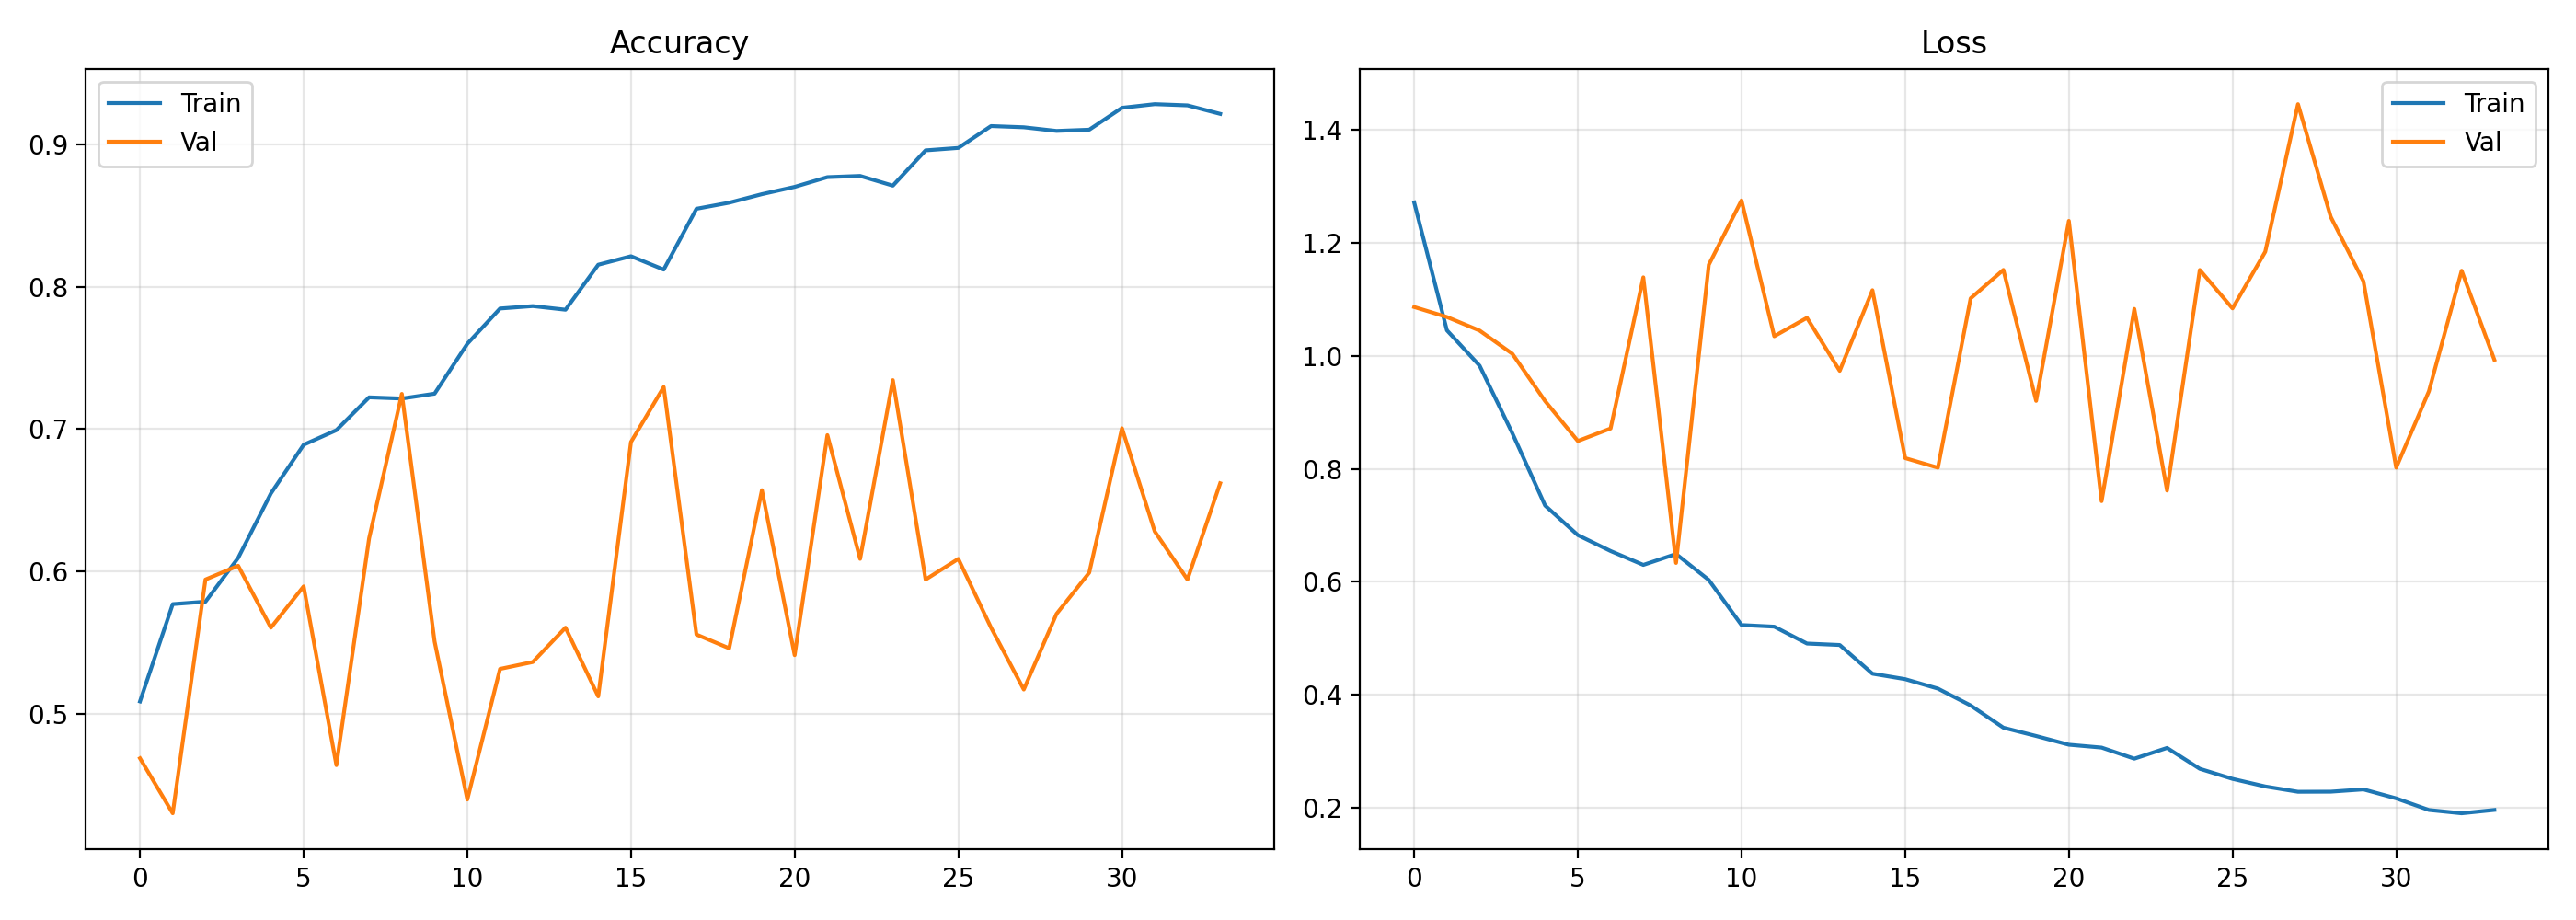
\includegraphics[width=0.95\textwidth]{training_history.png}
    \caption{Training and validation accuracy (left) and loss (right) over 35 epochs. Training accuracy steadily improves to $\sim$93\%, while validation accuracy fluctuates between 40--75\%, indicating some overfitting that is addressed by the ensemble approach.}
    \label{fig:training_history}
\end{figure}

\textbf{Observations from the training curves:}
\begin{itemize}
    \item The \textbf{training accuracy} increases monotonically from approximately 50\% to 93\% over 35 epochs, demonstrating that the model has sufficient capacity to learn the training data.
    \item The \textbf{training loss} decreases smoothly from 1.25 to approximately 0.20.
    \item The \textbf{validation accuracy} shows significant fluctuation (ranging between 40\% and 75\%), which is typical when training on small datasets with limited validation samples.
    \item The \textbf{validation loss} remains volatile (0.6--1.4), not decreasing as consistently as the training loss.
    \item The gap between training and validation performance indicates \textbf{overfitting}, which motivates the use of the ensemble approach.
\end{itemize}


\section{Single Model Performance}

The single best CNN model achieved a \textbf{test accuracy of 74.5\%}. While this demonstrates that the 1D CNN architecture can learn meaningful patterns from the 243-dimensional feature vector, the performance reveals specific challenges.

Figure~\ref{fig:confusion_single} shows the confusion matrix for the single model.

\begin{figure}[H]
    \centering
    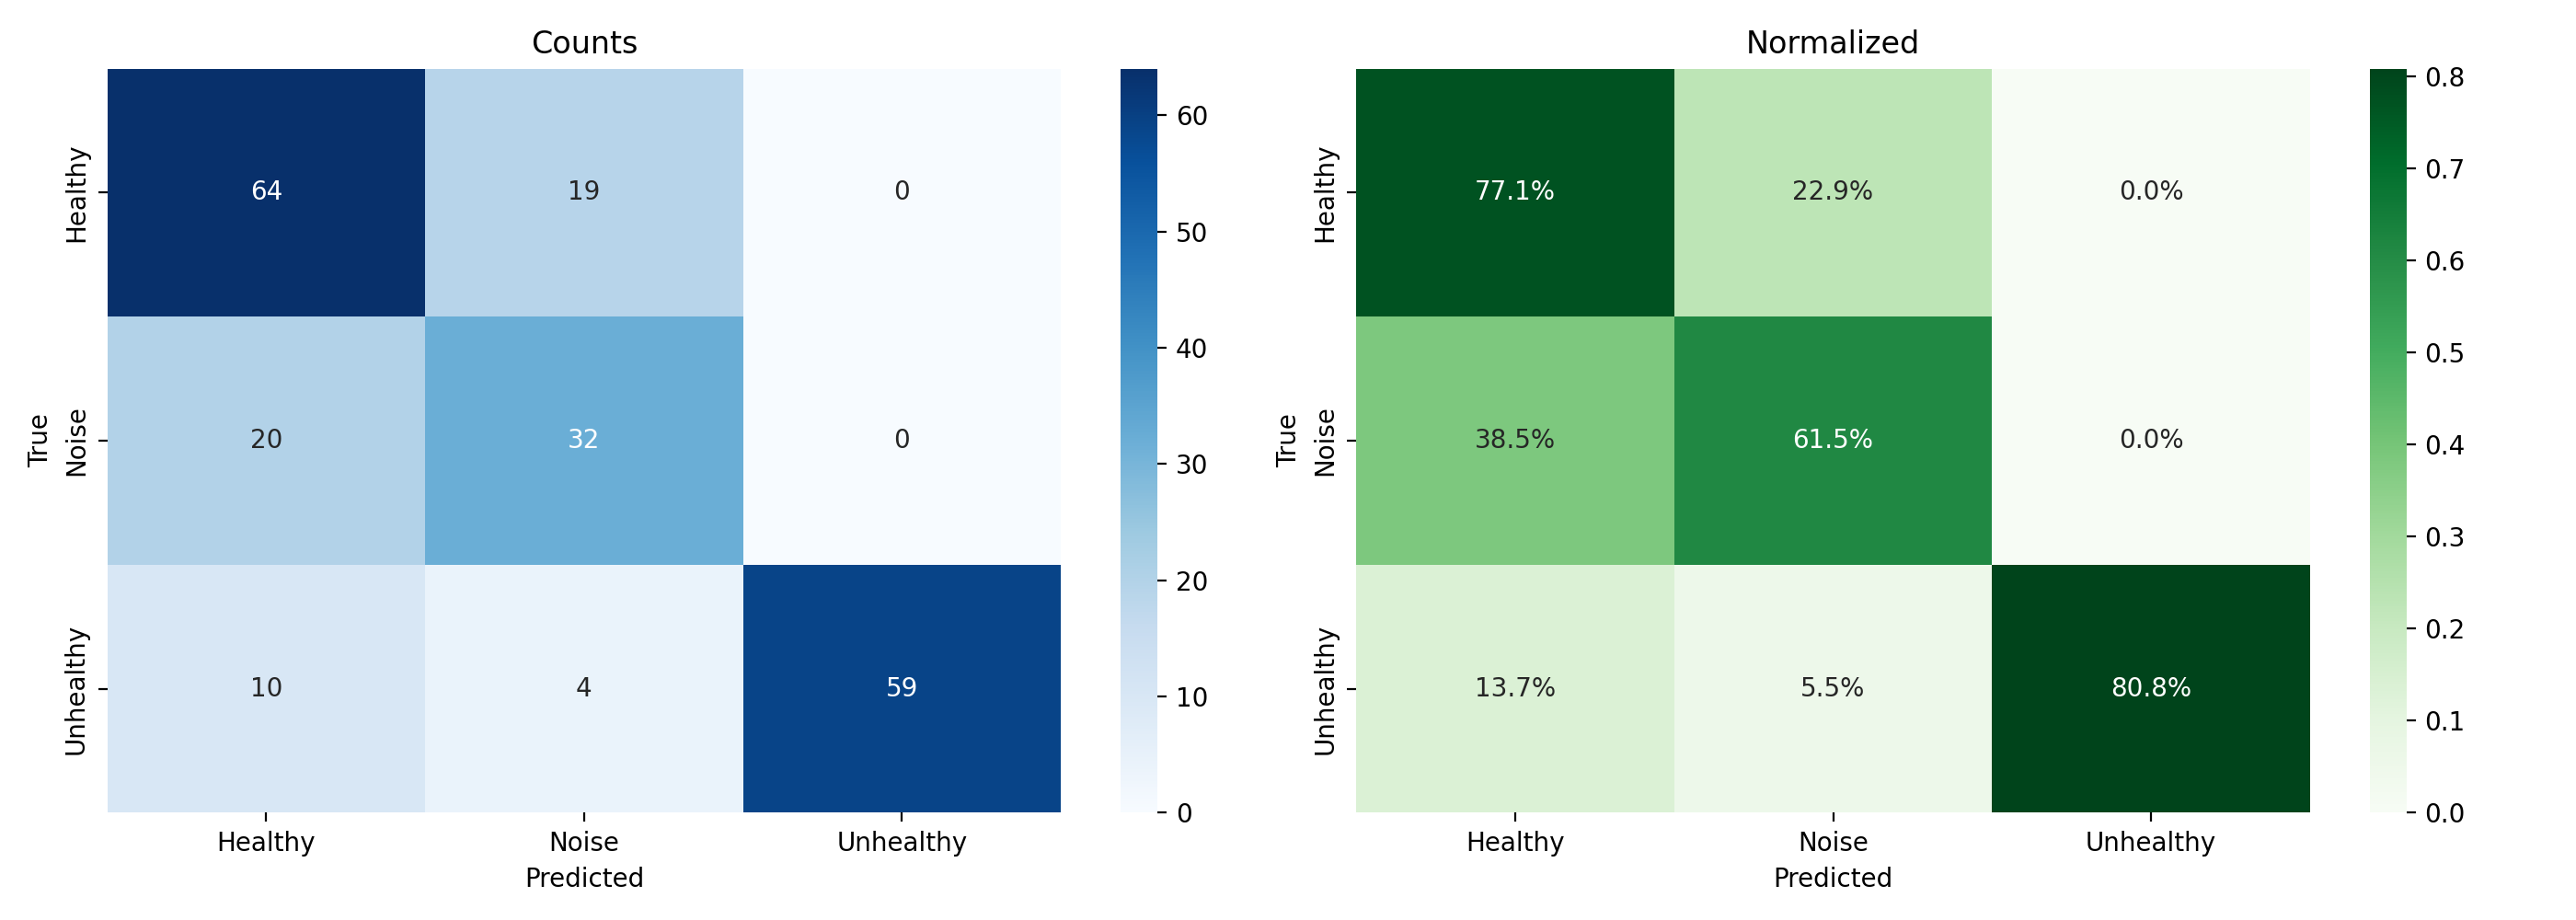
\includegraphics[width=0.95\textwidth]{confusion_matrix.png}
    \caption{Confusion matrix for the single CNN model (74.5\% accuracy). Left: raw counts. Right: normalized percentages. The Noise class shows the lowest recall at 61.5\%, with 38.5\% of Noise samples misclassified as Healthy.}
    \label{fig:confusion_single}
\end{figure}

\begin{table}[H]
\centering
\caption{Single model per-class performance.}
\label{tab:single_model_results}
\begin{tabular}{lccc}
\toprule
\textbf{True Class} & \textbf{Correct} & \textbf{Total} & \textbf{Recall} \\
\midrule
Healthy   & 64 & 83  & 77.1\% \\
Noise     & 32 & 52  & 61.5\% \\
Unhealthy & 59 & 73  & 80.8\% \\
\midrule
\textbf{Overall} & \textbf{155} & \textbf{208} & \textbf{74.5\%} \\
\bottomrule
\end{tabular}
\end{table}

\textbf{Key observations:}
\begin{itemize}
    \item The \textbf{Unhealthy} class achieves reasonably good recall (80.8\%), correctly identifying 59 out of 73 unhealthy samples.
    \item The \textbf{Noise} class has the lowest recall (61.5\%), with 20 out of 52 noise samples misclassified as Healthy. This confusion is understandable since some background noise in a poultry farm may contain ambient healthy chicken sounds.
    \item The \textbf{Healthy-Unhealthy confusion is minimal}: zero healthy samples were misclassified as unhealthy, and only 10 unhealthy samples were misclassified as healthy (13.7\%). This is a positive finding for the disease detection use case.
\end{itemize}


\section{Ensemble Model Performance}

The 3-model ensemble achieved a test accuracy of \textbf{92.8\%}, representing a significant improvement of \textbf{+18.3 percentage points} over the single model.

Figure~\ref{fig:confusion_ensemble} shows the ensemble confusion matrix.

\begin{figure}[H]
    \centering
    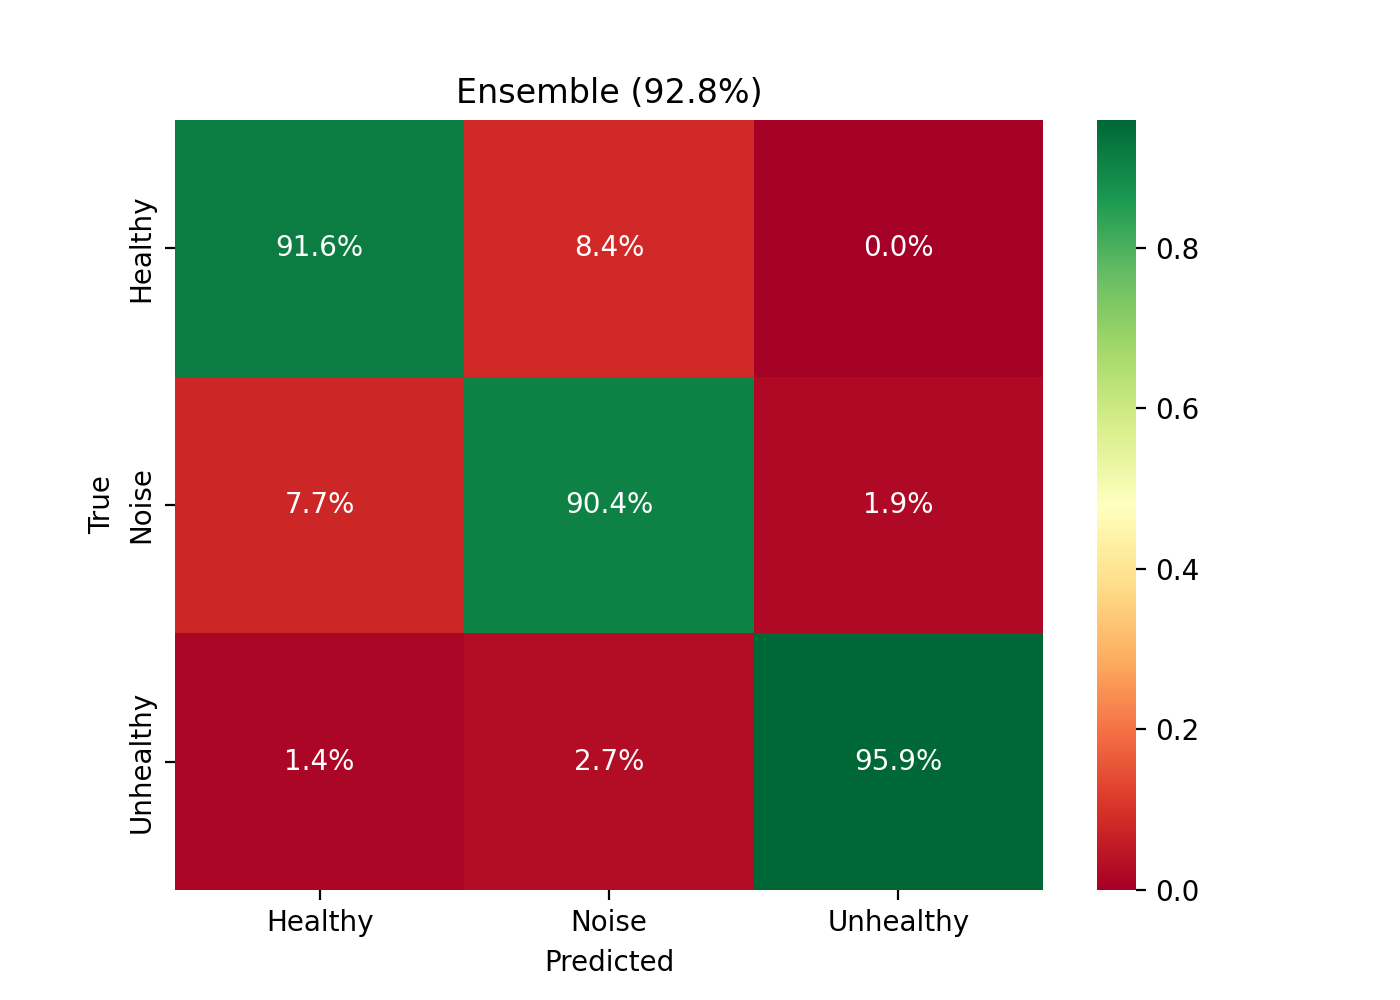
\includegraphics[width=0.65\textwidth]{ensemble_confusion.png}
    \caption{Confusion matrix for the 3-model ensemble (92.8\% accuracy). All three classes achieve recall above 90\%, with Unhealthy achieving the highest recall at 95.9\%.}
    \label{fig:confusion_ensemble}
\end{figure}

\begin{table}[H]
\centering
\caption{Ensemble model per-class performance.}
\label{tab:ensemble_results}
\begin{tabular}{lcccc}
\toprule
\textbf{True Class} & \textbf{Recall} & \multicolumn{3}{c}{\textbf{Predicted As}} \\
\cmidrule(l){3-5}
 & & Healthy & Noise & Unhealthy \\
\midrule
Healthy   & 91.6\% & \textbf{91.6\%} & 8.4\%  & 0.0\%  \\
Noise     & 90.4\% & 7.7\%           & \textbf{90.4\%} & 1.9\%  \\
Unhealthy & 95.9\% & 1.4\%           & 2.7\%  & \textbf{95.9\%} \\
\midrule
\multicolumn{2}{l}{\textbf{Overall Accuracy}} & \multicolumn{3}{c}{\textbf{92.8\%}} \\
\bottomrule
\end{tabular}
\end{table}


\section{Comparison: Single vs. Ensemble}

Table~\ref{tab:comparison} provides a direct comparison between the single model and the ensemble approach.

\begin{table}[H]
\centering
\caption{Performance comparison: Single model vs. 3-model ensemble.}
\label{tab:comparison}
\begin{tabular}{lccc}
\toprule
\textbf{Metric} & \textbf{Single Model} & \textbf{Ensemble} & \textbf{Improvement} \\
\midrule
Overall Accuracy   & 74.5\%  & \textbf{92.8\%}  & +18.3\% \\
Healthy Recall     & 77.1\%  & \textbf{91.6\%}  & +14.5\% \\
Noise Recall       & 61.5\%  & \textbf{90.4\%}  & +28.9\% \\
Unhealthy Recall   & 80.8\%  & \textbf{95.9\%}  & +15.1\% \\
\bottomrule
\end{tabular}
\end{table}

The ensemble approach provides dramatic improvements across all classes:
\begin{itemize}
    \item \textbf{Noise class:} The most dramatic improvement (+28.9\%), from 61.5\% to 90.4\%. The ensemble successfully resolves the Noise-Healthy confusion that plagued the single model.
    \item \textbf{Unhealthy class:} Achieves the highest recall at 95.9\%, which is critical since missing a diseased bird has the most serious consequences. Only 1.4\% of unhealthy samples are misclassified as healthy --- a very low false negative rate.
    \item \textbf{Healthy class:} Improves from 77.1\% to 91.6\%, with residual errors primarily being confusion with Noise (8.4\%), which is a relatively benign error.
\end{itemize}


\section{Analysis and Discussion}

\subsection{Why Ensemble Works}

The large gap between single model (74.5\%) and ensemble (92.8\%) performance can be attributed to several factors:

\begin{enumerate}
    \item \textbf{Variance reduction:} With only $\sim$344 samples and 243 features, a single model is prone to overfitting (as evidenced by the train-val gap in Figure~\ref{fig:training_history}). Averaging three models reduces this variance.
    \item \textbf{Error decorrelation:} Different random initializations cause models to learn different decision boundaries, so their errors tend to occur on different samples and partially cancel out.
    \item \textbf{Probability calibration:} Averaging softmax probabilities produces more calibrated confidence estimates than any individual model.
\end{enumerate}

\subsection{Error Analysis}

The remaining errors in the ensemble model (7.2\% overall error rate) primarily fall into three categories:
\begin{itemize}
    \item \textbf{Healthy $\to$ Noise (8.4\%):} Some healthy vocalizations may occur alongside significant background noise, leading to ambiguous classification. This error is the least concerning clinically.
    \item \textbf{Noise $\to$ Healthy (7.7\%):} Background noise in poultry farms often contains faint healthy vocalizations, making separation challenging.
    \item \textbf{Unhealthy $\to$ Noise/Healthy (4.1\%):} A small fraction of unhealthy samples are misclassified, possibly representing early-stage disease with subtle vocal changes.
\end{itemize}

Notably, \textbf{no healthy samples are classified as unhealthy} (0.0\%), meaning the system produces zero false alarms of disease from healthy vocalizations --- a highly desirable property for practical deployment.

\subsection{Feature Importance}

Based on the analysis conducted during development, the most discriminative features are:
\begin{itemize}
    \item \textbf{MFCC coefficients 1--5:} Capture the primary vocal tract characteristics that differ between healthy and diseased birds.
    \item \textbf{Power spectrum at 0.2 rad/sample:} Unhealthy signals exhibit a characteristic power spike at this frequency, corresponding to disease-related respiratory sounds.
    \item \textbf{Spectral contrast:} Healthy vocalizations show stronger harmonic structure (higher contrast) compared to the noisier spectra of diseased birds.
    \item \textbf{Delta MFCCs:} Temporal dynamics help distinguish transient disease sounds (coughs, rales) from sustained healthy vocalizations.
\end{itemize}


%%%%%%%%%%%%%%%%%%%%%%%%%%%%%%%%%%%%%%%%%%%%%%%%%%%%%%%%%%%%%%
% Chapter 6: Conclusion and Future Work
%%%%%%%%%%%%%%%%%%%%%%%%%%%%%%%%%%%%%%%%%%%%%%%%%%%%%%%%%%%%%%
\chapter{Conclusion and Future Work}
\label{ch:conclusion}

\section{Conclusion}

This project developed an automated system for early disease detection in chickens using audio-based deep learning. The key contributions and findings of this work are:

\begin{enumerate}
    \item \textbf{Comprehensive feature extraction:} A 243-dimensional feature vector was designed, encompassing MFCCs, Delta MFCCs, Chroma, Mel spectrogram statistics, Spectral Contrast, Tonnetz, spectral descriptors, autocorrelation, and statistical features. This represents a significant expansion over the 102-feature sets used in prior work.

    \item \textbf{Efficient preprocessing pipeline:} The combination of Hamming windowing and exponential low-pass filtering provides effective noise reduction at a fraction of the computational cost of Kalman filtering, making the system suitable for real-time processing.

    \item \textbf{1D CNN with ResNet and Attention:} A 1D Convolutional Neural Network incorporating residual skip connections and attention mechanisms was designed and trained for the 3-class classification task (Healthy, Noise, Unhealthy).

    \item \textbf{Ensemble for robustness:} A 3-model ensemble strategy was employed to address overfitting on the small dataset, boosting test accuracy from 74.5\% (single model) to \textbf{92.8\%} (ensemble) --- an improvement of 18.3 percentage points.

    \item \textbf{High disease detection recall:} The ensemble achieves \textbf{95.9\% recall} for the Unhealthy class and \textbf{0\% false alarm rate} from healthy vocalizations, demonstrating the system's reliability for disease detection.
\end{enumerate}

The results demonstrate that audio-based deep learning is a viable and effective approach for non-invasive poultry health monitoring. The system can operate continuously without disturbing the birds, providing a scalable solution for modern poultry farms.

\section{Future Work}

Several directions for future research and system improvement have been identified:

\begin{itemize}
    \item \textbf{Larger dataset:} Expanding the dataset beyond 344 samples through additional field recordings and data augmentation techniques (time stretching, pitch shifting, noise injection) would improve model generalization and reduce the need for ensemble approaches.

    \item \textbf{Real-time deployment:} Developing an edge computing solution (e.g., running on a Raspberry Pi with a microphone array) for continuous, real-time monitoring in poultry houses. This would require optimizing the model through techniques such as quantization and pruning.

    \item \textbf{Disease-specific classification:} Extending the Unhealthy class into specific disease categories (e.g., infectious bronchitis, Mycoplasma, Newcastle disease) to provide more actionable diagnostic information.

    \item \textbf{Multi-modal integration:} Combining audio analysis with other sensors (temperature, humidity, video) to create a more comprehensive health monitoring system.

    \item \textbf{Temporal modeling:} Incorporating sequence models (e.g., LSTM or Transformer) to analyze how vocalizations change over time, potentially enabling detection of disease progression.

    \item \textbf{Transfer learning:} Exploring pre-trained audio models (such as YAMNet or VGGish) and fine-tuning them on the poultry vocalization domain, which may yield better feature representations even with limited training data.

    \item \textbf{Model interpretability:} Applying techniques such as Grad-CAM or SHAP analysis to better understand which features the CNN ensemble relies on for its predictions, increasing trust and adoption among poultry farm operators.
\end{itemize}


%%%%%%%%%%%%%%%%%%%%%%%%%%%%%%%%%%%%%%%%%%%%%%%%%%%%%%%%%%%%%%
% References
%%%%%%%%%%%%%%%%%%%%%%%%%%%%%%%%%%%%%%%%%%%%%%%%%%%%%%%%%%%%%%
\clearpage
\addcontentsline{toc}{chapter}{References}
\begin{thebibliography}{9}

\bibitem{datainbrief2023}
\textit{Poultry Vocalization Signal Dataset.} Data in Brief, Volume 50, 109528, 2023. Dataset with Hamming windowing and Kalman filter preprocessing for poultry health audio analysis.

\bibitem{chen2016xgboost}
Chen, T., \& Guestrin, C. (2016). XGBoost: A Scalable Tree Boosting System. In \emph{Proceedings of the 22nd ACM SIGKDD International Conference on Knowledge Discovery and Data Mining} (pp. 785--794). ACM.

\bibitem{he2016resnet}
He, K., Zhang, X., Ren, S., \& Sun, J. (2016). Deep Residual Learning for Image Recognition. In \emph{Proceedings of the IEEE Conference on Computer Vision and Pattern Recognition (CVPR)} (pp. 770--778).

\end{thebibliography}

\end{document}
